\documentclass[tikz,border=4pt]{standalone}
\usepackage{amsmath}
\usepackage{pgfplots}
\pgfplotsset{compat=1.18}

\begin{document}
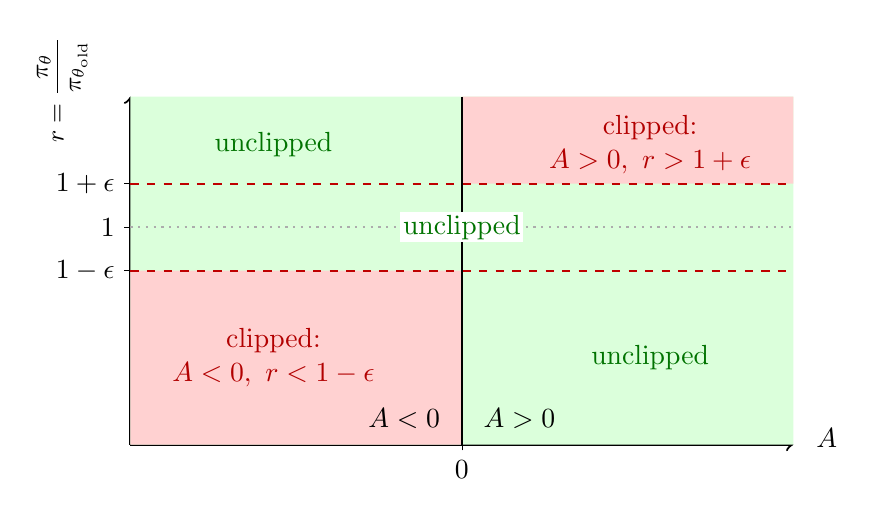
\begin{tikzpicture}
\begin{axis}[
  width=10cm,
  height=6cm,
  xmin=-2.2,
  xmax=2.2,
  ymin=0,
  ymax=1.6,
  axis lines=left,
  axis line style={->, thick},
  xlabel={$A$},
  ylabel={$r=\dfrac{\pi_\theta}{\pi_{\theta_{\mathrm{old}}}}$},
  xlabel style={at={(axis description cs:1.02,0.02)}, anchor=west},
  ylabel style={at={(axis description cs:-0.05,1.02)}, anchor=south, font=\small},
  xtick={0},
  xticklabels={$0$},
  ytick={0.8,1,1.2},
  yticklabels={$1-\epsilon$,$1$,$1+\epsilon$},
  tick style={black},
  enlargelimits=false,
  clip=false
]

% Green: the minimum keeps the original ratio term rA.
\addplot[draw=none, fill=green!14] coordinates
  {(-2.2,0) (2.2,0) (2.2,1.6) (-2.2,1.6)} \closedcycle;

% Regions where the PPO clipped objective uses the clipped ratio.
\addplot[draw=none, fill=red!18] coordinates
  {(0,1.2) (2.2,1.2) (2.2,1.6) (0,1.6)} \closedcycle;
\addplot[draw=none, fill=red!18] coordinates
  {(-2.2,0) (0,0) (0,0.8) (-2.2,0.8)} \closedcycle;

\addplot[red!75!black, dashed, thick] coordinates {(-2.2,0.8) (2.2,0.8)};
\addplot[red!75!black, dashed, thick] coordinates {(-2.2,1.2) (2.2,1.2)};
\addplot[gray!65, dotted, thick] coordinates {(-2.2,1) (2.2,1)};
\addplot[black, thick] coordinates {(0,0) (0,1.6)};

\node[align=center, text=green!45!black, fill=white, inner sep=1pt] at (axis cs:0,1.0)
  {unclipped};
\node[align=center, text=red!70!black] at (axis cs:1.25,1.38)
  {clipped:\\ $A>0,\ r>1+\epsilon$};
\node[align=center, text=red!70!black] at (axis cs:-1.25,0.4)
  {clipped:\\ $A<0,\ r<1-\epsilon$};
\node[align=center, text=green!45!black] at (axis cs:-1.25,1.38)
  {unclipped};
\node[align=center, text=green!45!black] at (axis cs:1.25,0.4)
  {unclipped};
\node[anchor=west] at (axis cs:0.08,0.12)
  {$A>0$};
\node[anchor=east] at (axis cs:-0.08,0.12)
  {$A<0$};

\end{axis}
\end{tikzpicture}
\end{document}
